\documentclass[reprint,aps,unsortedaddress,superscriptaddress,prc,floatfix,showpacs,linenumbers,final]{revtex4-2}
\usepackage[utf8]{inputenc}
\usepackage{float}
\usepackage{graphicx}
\usepackage{amsmath,amsthm,amssymb}
\usepackage{verbatim}
\usepackage{url}
\usepackage{subcaption}
\usepackage[separate-uncertainty=true]{siunitx}
\usepackage{physics}
\usepackage[pdfusetitle]{hyperref}
\usepackage[capitalize]{cleveref}
\usepackage[obeyFinal]{todonotes}
\setuptodonotes{inline}
\usepackage{adjustbox}
\usepackage{multirow}
\usepackage{lineno}
\usepackage{cmap}
\usepackage[version=4]{mhchem}
\usepackage{makecell}
\linenumbers
\graphicspath{{figures/}}
\DeclareSIUnit\barn{b}

\captionsetup{justification=raggedright,singlelinecheck=false}

\usepackage[most]{tcolorbox}

%\let\includegraphicsold\includegraphics
%\renewcommand{\includegraphics}[2][]{\tcbox{\includegraphicsold[#1]{#2}}}

\begin{document}

\title{Improved measurement of flavor asymmetry of the light-quark sea in the proton with Drell-Yan production in
	\texorpdfstring{$p+p$}{p+p} and \texorpdfstring{$p+d$}{p+d} collisions at \texorpdfstring{\SI{120}{\GeV}}{120~GeV}}
% !TeX root = main.tex
\author{C.~H.~Leung}
\affiliation{Department of Physics, University of Illinois at Urbana-Champaign, Urbana, Illinois 61801, USA}

\author{J.~C.~Peng}
\affiliation{Department of Physics, University of Illinois at Urbana-Champaign,
Urbana, Illinois 61801, USA}

\begin{comment}
\author{J. Dove}
\affiliation{Department of Physics, University of Illinois at Urbana-Champaign,
Urbana, Illinois 61801, USA}

\author{B.~Kerns}
\affiliation{Department of Physics, University of Illinois at Urbana-Champaign,
Urbana, Illinois 61801, USA}

\author{R.~E.~McClellan}
\altaffiliation[Present address ]{Pensacola State College, Pensacola, FL 32504}
\affiliation{Department of Physics, University of Illinois at Urbana-Champaign, 
Urbana, Illinois 61801, USA}

\author{S.~Miyasaka}
\affiliation{Department of Physics, Tokyo Institute of Technology, Meguro-ku, Tokyo 152-8550, Japan}

\author{D.~H.~Morton}
\affiliation{Randall Laboratory of Physics, University of Michigan, Ann Arbor,
Michigan 48109, USA}

\author{K.~Nagai}
\affiliation{Department of Physics, Tokyo Institute of Technology, Meguro-ku, Tokyo 152-8550, Japan}
\affiliation{Institute of Physics, Academia Sinica, Taipei, 11529, Taiwan}
\affiliation{Physics Division, Los Alamos National Laboratory, Los Alamos, New Mexico 97545, USA}

\author{S.~Prasad}
\affiliation{Department of Physics, University of Illinois at Urbana-Champaign,
Urbana, Illinois 61801, USA}
\affiliation{Physics Division, Argonne National Laboratory, Lemont, Illinois 60439, USA}

\author{F.~Sanftl}
\affiliation{Department of Physics, Tokyo Institute of Technology, Meguro-ku,
Tokyo 152-8550, Japan}

\author{M.~B.~C.~Scott}
\affiliation{Randall Laboratory of Physics, University of Michigan, Ann Arbor,Michigan 48109, USA}
\affiliation{Physics Division, Argonne National Laboratory, Lemont, Illinois 60439, USA}

\author{A.~S.~Tadepalli}
\altaffiliation[Present address ]{Thomas Jefferson National Accelerator Facility, Newport News, Virginia 23606, USA}
\affiliation{Department of Physics and Astronomy, Rutgers, The State University of New Jersey, Piscataway, New Jersey 08854, USA}

\author{C.~A.~Aidala}
\affiliation{Randall Laboratory of Physics, University of Michigan, Ann Arbor, Michigan 48109, USA}
\affiliation{Physics Division, Los Alamos National Laboratory, Los Alamos, New Mexico 87545, USA}

\author{J.~ Arrington}
\altaffiliation[Present address ]{Lawrence Berkeley National Laboratory, Berkeley, California, 94720 USA}
\affiliation{Physics Division, Argonne National Laboratory, Lemont, Illinois 60439, USA}

\author{C.~Ayuso}
\affiliation{Randall Laboratory of Physics, University of Michigan, Ann Arbor,
Michigan 48109, USA}

\author{C.~T.~Barker}
\affiliation{Department of Engineering and Physics, Abilene Christian University, Abilene, Texas 79699, USA}

\author{C.~N.~Brown}
\affiliation{Fermi National Accelerator Laboratory, Batavia, Illinois 60510, USA}

\author{T.~H.~Chang}
\affiliation{Institute of Physics, Academia Sinica, Taipei, 11529, Taiwan}

\author{W.~C.~Chang}
\affiliation{Institute of Physics, Academia Sinica, Taipei, 11529, Taiwan}

\author{A.~Chen}
\affiliation{Department of Physics, University of Illinois at Urbana-Champaign, Urbana, Illinois 61801, USA}
\affiliation{Institute of Physics, Academia Sinica, Taipei, 11529, Taiwan}
\affiliation{Randall Laboratory of Physics, University of Michigan, Ann Arbor, Michigan 48109, USA}

\author{D.~C.~Christian}
\affiliation{Fermi National Accelerator Laboratory, Batavia, Illinois 60510, USA}

\author{B.~P.~Dannowitz}
\affiliation{Department of Physics, University of Illinois at Urbana-Champaign, Urbana, Illinois 61801, USA}

\author{M.~Daugherity}
\affiliation{Department of Engineering and Physics, Abilene Christian University, Abilene, Texas 79699, USA}

\author{M.~Diefenthaler}
\affiliation{Department of Physics, University of Illinois at Urbana-Champaign, Urbana, Illinois 61801, USA}

\author{L.~El Fassi}
\affiliation{Department of Physics and Astronomy, Mississippi State University, Mississippi State, Mississippi 39762, USA }
\affiliation{Department of Physics and Astronomy, Rutgers, The State University of New Jersey, Piscataway, New Jersey 08854, USA}

\author{D.~F.~Geesaman}
\affiliation{Physics Division, Argonne National Laboratory, Lemont, Illinois 60439, USA}

\author{R.~Gilman}
\affiliation{Department of Physics and Astronomy, Rutgers, The State University of New Jersey, Piscataway, New Jersey 08854, USA}

\author{Y.~Goto}
\affiliation{RIKEN Nishina Center for Accelerator-Based Science, Wako, Saitama 351-0198, Japan}

\author{L.~Guo}
\altaffiliation[Present address ]{Florida International University, Miami, Florida, 33199, USA}
\affiliation{Physics Division, Los Alamos National Laboratory, Los Alamos, New Mexico 87545, USA}

\author{R.~Guo}
\affiliation{Department of Physics, National Kaohsiung Normal University, Kaohsiung City 80201, Taiwan}

\author{T.~J.~Hague}
\altaffiliation[Present address ]{Lawrence Berkeley National Laboratory, Berkeley, California, 94720 USA}
\affiliation{Department of Engineering and Physics, Abilene Christian University, Abilene, Texas 79699, USA}

\author{R.~J.~Holt}
\altaffiliation[Present address ]{Kellogg Radiation Laboratory, California Institute of Technology, Pasadena, California 91125, USA}
\affiliation{Physics Division, Argonne National Laboratory, Lemont, Illinois 60439, USA}

\author{D.~Isenhower}
\affiliation{Department of Engineering and Physics, Abilene Christian University, Abilene, Texas 79699, USA}

\author{E.~R.~Kinney}
\affiliation{Department of Physics, University of Colorado, Boulder,
Colorado 80309, USA}

\author{N.~D.~Kitts}
\affiliation{Department of Engineering and Physics, Abilene Christian University, Abilene, Texas 79699, USA}

\author{A.~Klein}
\affiliation{Physics Division, Los Alamos National Laboratory, Los Alamos, New Mexico 87545, USA}

\author{D.~W.~Kleinjan}
\affiliation{Physics Division, Los Alamos National Laboratory, Los Alamos, New Mexico 87545, USA}

\author{Y.~Kudo}
\affiliation{Department of Physics, Yamagata University, Yamagata City, Yamagata 990-8560, Japan}

\author{P.-J.~Lin}
\affiliation{Department of Physics, University of Colorado, Boulder, Colorado 80309, USA}
\affiliation{Institute of Physics, Academia Sinica, Taipei, 11529, Taiwan}

\author{K.~Liu}
\affiliation{Physics Division, Los Alamos National Laboratory, Los Alamos, New Mexico 87545, USA}

\author{M.~X.~Liu}
\affiliation{Physics Division, Los Alamos National Laboratory, Los Alamos,
New Mexico 87545, USA}

\author{W.~Lorenzon}
\affiliation{Randall Laboratory of Physics, University of Michigan, Ann Arbor,
Michigan 48109, USA}

\author{N.~C.~R.~Makins}
\affiliation{Department of Physics, University of Illinois at Urbana-Champaign, Urbana, Illinois 61801, USA}

\author{M.~Mesquita de Medeiros}
\affiliation{Physics Division, Argonne National Laboratory, Lemont,
Illinois 60439, USA}

\author{P.~L.~McGaughey}
\affiliation{Physics Division, Los Alamos National Laboratory, Los Alamos,
New Mexico 87545, USA}

\author{Y.~Miyachi}
\affiliation{Department of Physics, Yamagata University, Yamagata City,
Yamagata 990-8560, Japan}

\author{I.~Mooney}
\altaffiliation[Present address ]{Wayne State University, Detroit, MI 48202, USA}
\affiliation{Randall Laboratory of Physics, University of Michigan, Ann Arbor, Michigan 48109, USA}

\author{K.~Nakahara}
\altaffiliation[Present address ]{Stanford Linear Accelerator Center, Menlo Park, CA 94025, USA}
\affiliation{Department of Physics, University of Maryland, College Park, Maryland 20742, USA}

\author{K.~Nakano}
\affiliation{University of Virginia, Charlottesville, Virginia 22904, USA}
\affiliation{Department of Physics, Tokyo Institute of Technology, Meguro-ku, Tokyo 152-8550, Japan}
\affiliation{RIKEN Nishina Center for Accelerator-Based Science, Wako, Saitama 351-0198, Japan}

\author{S.~Nara}
\affiliation{Department of Physics, Yamagata University, Yamagata City, Yamagata 990-8560, Japan}


\author{A.~J.~Puckett}
\altaffiliation[Present address ]{University of Connecticut, Storrs, CT 06269, USA}
\affiliation{Physics Division, Los Alamos National Laboratory, Los Alamos, New Mexico 87545, USA}

\author{B.~J.~Ramson}
\affiliation{Randall Laboratory of Physics, University of Michigan, Ann Arbor, Michigan 48109, USA}
\affiliation{Fermi National Accelerator Laboratory, Batavia, Illinois 60510, USA}

\author{P.~E.~Reimer}
\affiliation{Physics Division, Argonne National Laboratory, Lemont, Illinois 60439, USA}

\author{J.~G.~Rubin}
\affiliation{Randall Laboratory of Physics, University of Michigan, Ann Arbor, Michigan 48109, USA}
\affiliation{Physics Division, Argonne National Laboratory, Lemont, Illinois 60439, USA}

\author{S.~Sawada}
\affiliation{Institute of Particle and Nuclear Studies, KEK, High Energy Accelerator Research Organization, Tsukuba, Ibaraki 305-0801, Japan}

\author{T.~Sawada}
\altaffiliation[Present address ]{Nambu Yoichiro Institute of Theoretical and Experimental Physics, Osaka Metropolitan University, Osaka 558-8585, JAPAN}
\affiliation{Randall Laboratory of Physics, University of Michigan, Ann Arbor, Michigan 48109, USA}

\author{T.-A.~Shibata}
\altaffiliation[Present address ]{Nihon University, College of Science and Technology, Chiyoda-ku, Tokyo 101-8308, Japan}
\affiliation{Department of Physics, Tokyo Institute of Technology, Meguro-ku, Tokyo 152-8550, Japan}
\affiliation{RIKEN Nishina Center for Accelerator-Based Science, Wako, Saitama 351-0198, Japan}

\author{S.~H.~Shiu}
\affiliation{Institute of Physics, Academia Sinica, Taipei, 11529, Taiwan}

\author{D.~Su}
\affiliation{Institute of Physics, Academia Sinica, Taipei, 11529, Taiwan}

\author{M.~Teo}
\affiliation{Department of Physics, University of Illinois at Urbana-Champaign, Urbana, Illinois 61801, USA}

\author{B.~G Tice}
\affiliation{Physics Division, Argonne National Laboratory, Lemont, Illinois 60439, USA}

\author{R.~S.~Towell}
\affiliation{Department of Engineering and Physics, Abilene Christian University, Abilene, Texas 79699, USA}

\author{S.~Uemura}
\altaffiliation[Present address ]{Fermi National Accelerator Laboratory, Batavia, Illinois 60510, USA}
\affiliation{Department of Engineering and Physics, Abilene Christian University, Abilene, Texas 79699, USA}

\author{T.~S.~Watson}
\affiliation{Department of Engineering and Physics, Abilene Christian University, Abilene, Texas 79699, USA}

\author{S.~G.~Wang}
\altaffiliation[Present address ]{APS, Argonne National Laboratory, Lemont, Illinois 60439, USA}
\affiliation{Institute of Physics, Academia Sinica, Taipei, 11529, Taiwan}
\affiliation{Department of Physics, National Kaohsiung Normal University, Kaohsiung City 80201, Taiwan}

\author{A.~B.~Wickes}
\affiliation{Physics Division, Los Alamos National Laboratory, Los Alamos,
New Mexico 87545, USA}

\author{J.~Wu}
\affiliation{Fermi National Accelerator Laboratory, Batavia, Illinois 60510, USA}

\author{Z.~Xi}
\affiliation{Department of Engineering and Physics, Abilene Christian University, Abilene, Texas 79699, USA}

\author{Z.~Ye}
\altaffiliation[Present address ]{Department of Physics, Tsinghua University, Beijing 100084 China}
\affiliation{Physics Division, Argonne National Laboratory, Lemont, Illinois 60439, USA}
\end{comment}
\author{Others...}
\collaboration{FNAL E906/SeaQuest Collaboration}
%\noaffiliation


\date{\today}

\begin{abstract}
	We report improved results from the SeaQuest Fermilab E906 experiment with improved statistical precision for
	$\bar{d}\left(x\right) / \bar{u}\left(x\right)$ in the large $x$ region up to $x=0.45$ using the 120 GeV proton beam.
	The $\bar{d}\left(x\right) / \bar{u}\left(x\right)$ ratios and the $\bar{d}\left(x\right) - \bar{u}\left(x\right)$
	differences are deduced from these cross section ratios for $0.13 < x < 0.45$.
	The new results on $\bar{d}\left(x\right) / \bar{u}\left(x\right)$ and $\bar{d}\left(x\right) - \bar{u}\left(x\right)$
	are compared with various parton distribution functions and theoretical calculations.
\end{abstract}


\maketitle

\section{Introduction}
The large asymmetry of the distributions of $\bar{d}$ and $\bar{u}$ in the proton was first observed in deep inelastic
scattering experiments via the violation of the Gottfried sum rule~\cite{amaudruz1991}. 
The Bjorken-$x$ dependence of this light sea-quark asymmetry measured the FNAL E866/NuSea
experiment using the Drell-Yan process~\cite{towell2001}.
The small-$x$ region has been measured with high precision by E866,
using an \SI{800}{\GeV} proton beam. 
The FNAL E906/SeaQuest experiment, using a new spectrometer~\cite{aidala2019} and a \SI{120}{\GeV}
proton beam, has extended the measurement to higher $x$~\cite{dove2021,dove2023}. 
%\todo{are we comparing with E866 here?}
%\todo{summarized previos finding?}
%\todo{discribe the results from STAR and why this new result is better}
Results on the charmonium production have also been reported recently in Ref.~\cite{leung2024a}.
The SeaQuest data is separated into two sets, each roughly half of the data sample.
The first part covers the data taken between June 2014 and July 2015.
Results from the analysis of the first part of data have been reported in the earlier work~\cite{dove2021,dove2023}, 
and we have shown that the $\sigma_{pd}/2\sigma_{pp}$ ratio to remain above one.
Therefore suggesting $\bar{d}/\bar{u}$ ratio to remain above unity in the proton,
contrary to the results from E866~\cite{towell2001}.
Several recent global PDF analyses~\cite{cocuzza2021,ball2022a,accardi2023,alekhin2023}
have included these results, in addition to the $W$ boson production data from the STAR collaboration~\cite{adam2021}.
The second set of data covers the remaining period up to July 2016.
In this paper, we report the improved results on the Drell-Yan measurements
by including both sets of data collected by the SeaQuest Experiment at Fermilab.
The data constitute a two-fold increase in the detected muons compared to our previous publications.
Since the trigger
conditions and the detector configuration for the two data sets are not
identical, the analysis was performed separately for each data set. 
Results obtained from the two data sets are first compared to verify their
consistency, and then combined for the final results.
%\todo{also summarized any improvement in the analysis if any}


Several models, including the meson cloud model~\cite{alberg2022} and statistical model~\cite{soffer2019},
have been proposed to explain the light sea-quark asymmetry.
Recent advancement in lattice QCD allows the partonic structure to be calculated within the LaMET framework~\cite{constantinou2021}.
The SeaQuest measurement of the Drell-Yan cross section ratio at large $x_2$ can provide strong
constrains on the flavor asymmetry and checks the various models.

After this introduction, the Drell-Yan process and the kinematic variables are briefly summarized in \cref{sec:drell-yan}.
The SeaQuest experiment is described in \cref{sec:seaquest_spectrometer}.
\Cref{sec:analysis} presents the data analysis.
Results of the Drell-Yan cross section ratios are presented in \cref{sec:csr}.
\Cref{sec:extraction} discusses the extraction of the $\bar{d}/\bar{u}$ and $\bar{d}-\bar{u}$
from the measured ratios.
The results on the absolute Drell-Yan cross section are presented in \cref{sec:abs_cs}.
We conclude in \cref{sec:Conclusions}.

\section{The Drell-Yan Process}
\label{sec:drell-yan}
The SeaQuest experiment detects $\mu^+\mu^-$ pairs (dimuons) produced in the interaction of a proton
beam with various targets nuclei. The production of massive dimuon pairs are described by the Drell-Yan
process~\cite{drell1970}. In the Drell-Yan process, the leading order (LO) cross section is given by
\begin{multline}
	\frac{d^2\sigma}{dx_1dx_2}=\frac{4\pi \alpha^2}{9x_1x_2s} \times
	\label{eq:DYCross} \\
	\sum_{i\in u,d,s,\dots} e_i^2 \left[q_i^A\left(x_1\right) \bar q_i^B\left(x_2\right) + \bar q_i^A\left(x_1\right)
		q_i^B\left(x_2\right)\right],
\end{multline}
where $\alpha$ is the fine-structure constant, $e_i$ is the charge of a quark with flavor $i$,
and $q_i^{A,B}\left(x_{1,2}\right)$ are the quark distribution functions in hadrons $A$ and $B$
for quarks carrying a momentum fraction $x_1$ and $x_2$, respectively.
An analogous notation is used for antiquark distribution functions $\bar q_i^{A,B}\left(x_{1,2}\right)$.

The experiment measures the momenta of the $\mu^+$ and $\mu^-$, $p_{\mu^+}$ and $p_{\mu^-}$.
From these, the four-momentum $Q$ of virtual photon from the quark-antiquark annihilation is determined,
$Q = p_{\mu^+} + p_{\mu^-}$.
The variables $x_1$ and $x_2$ of the quark-antiquark pair are then
\begin{equation}
	x_1 = \frac{P_2 \cdot Q}{P_2 \cdot P} \text{ and } x_2 =
	\frac{P_1 \cdot Q}{P_1 \cdot P},
	\label{def_x1x2}
\end{equation}
where $P_1$ and $P_2$ are the four-momenta of the projectile and target hadron,
respectively, and $P$ is the sum of $P_1$ and $P_2$, $P=P_1+P_2$.
The invariant mass-squared of the dimuon, $M^2 = Q^2$, is related to $x_1$, $x_2$, $s$, and $P_T$ by
\begin{equation}
	M^2=x_1 x_2 s - P_T^2,
	\label{def_mass}
\end{equation}
where $P_T$ is the transverse momentum of the dimuon.

The Feynman-$x$, $x_F$, of the dimuon is
\begin{equation}
	x_F = \frac{P_L}{P_{\text{max}}} = \frac{2P_L}{\sqrt{s}\left(1-M^2/s\right)},
	\label{def_xf}
\end{equation}
where $P_L$ is the longitudinal momentum of the dimuon and $P_\textrm{max}$ is the maximum momentum in the center-of-mass frame of the colliding hadrons.
With the definition of $x_F$ adopted in \cref{def_xf},
the full range of $\left|x_F\right| < 1$ is covered.
In contrast, for the alternative definition of $x_F = 2P_L/\sqrt{s}$,
frequently used in the literature,
the coverage of $x_F$ is limited to $\left|x_F\right| <\left(1-M^2/s\right)$.
These two definitions of $x_F$ converge at the high-energy limit when $M^2/s \to 0$.
It is worth noting that \cref{def_mass} becomes the familiar expression $M^2=x_1 x_2 s$,
often adopted in the literature, when $P_T/\sqrt{s} \to 0$.
For the SeaQuest experiment, the modest beam momentum of \SI{120}{\GeV} $\left(\sqrt{s} = \SI{15.1}{\GeV}\right)$
warrants the use of the definitions of kinematic variables shown in \cref{def_mass} and \ref{def_xf}.

The leading order Drell-Yan cross section, expressed in \cref{eq:DYCross},
contains two terms since the annihilation could proceed with the antiquark from either parent hadron.
For most fixed-target experiments, including SeaQuest,
the spectrometers have large acceptance for the positive $x_F$  region $\left(x_F > 0\right)$.
Thus, to a good approximation, the Drell-Yan cross section is dominated by the first term,
corresponding to the annihilation of a beam quark with a target antiquark.
To demonstrate the relation between the cross section ratio and the flavor asymmetry
$\bar{d}\left(x\right) / \bar{u}\left(x\right)$,
an approximate formula can be derived as follows.
Taking into account the dominance of $u\left(x\right)$ over $d\left(x\right)$ in
beam proton and the charge squared weighting factor $e_i^2$ in \cref{eq:DYCross}, one obtains for $x_1 \gg x_2$,
\begin{align}
	\frac{\sigma^{pd}}{2\sigma^{pp}} = \frac{1}{2}\left[1 + \frac{\sigma^{pn}}{\sigma^{pp}}\right]
	\approx \frac{1}{2}\left[1 + \frac{\bar{u}_n\left(x_2\right)}{\bar{u}_p\left(x_2\right)}\right],
\end{align}
with the assumption that $\sigma^{pd} \approx \sigma^{pp} + \sigma^{pn}$,
which neglects small nuclear effects of the deuteron~\cite{kumano1998,ehlers2014}.
Charge symmetry for the parton distributions~\cite{londergan2010} between the proton and the neutron:
\begin{equation}
	\begin{split}
		\bar u\left(x\right)  \equiv & \bar u_p\left(x\right) = \bar d_n\left(x\right)\textrm{, and } \\
		\bar d\left(x\right)  \equiv & \bar d_p\left(x\right) = \bar u_n\left(x\right),
	\end{split}
	\label{eq:chargeSymmetry}
\end{equation}
leads to the approximate expression
\begin{equation}
	\frac{\sigma^{pd}}{2\sigma^{pp}} \approx
	\frac{1}{2} \left[1+\frac{\bar d\left(x_2\right)}{\bar u\left(x_2\right)}\right].
	\label{eq:crRatio}
\end{equation}
While \cref{eq:crRatio} illustrates the power of the $\sigma^{pd}/2\sigma^{pp}$ Drell-Yan cross section
ratio to reveal the flavor asymmetry between $\bar d$ and $\bar u$,
the actual extraction of the $\bar d\left(x\right) / \bar u\left(x\right)$ ratios
from the measured $\sigma^{pd}/ 2 \sigma^{pp}$ Drell-Yan cross section ratios is
made without these simplifying approximations and is carried out in Next-to-Leading Order (NLO)
in the strong coupling constant, $\alpha_s$, as discussed in Sec.~\ref{sec:extraction}.

\section{The SeaQuest Experiment}
\label{sec:seaquest_spectrometer}
The SeaQuest experiment receives the  proton beam from the Fermilab Main Injector at \SI{120}{\GeV}
once every minute in 4-second periods (spills).
The proton beam is further grouped into \SI{2}{\ns} ``buckets'' every \SI{18.8}{\ns},
inherited from the accelerator \SI{53.1}{\MHz} radiofrequency (RF) structure.
The average intensity of the beam is approximately $2\times 10^{12}$ protons per second.
The proton beam in the Main Injector are peeled off using a process known as resonance
extraction over the course of the \SI{4}{\second} spill.
While the average instantaneous intensity was roughly $10^4$ protons per buckets,
the measured numbers varied up to few times of $10^5$ protons.

Buckets with a large number of protons can produce large numbers of hits in the detector,
easily satisfy the trigger requirements, and can saturate the data
Moreover, these events are typically too noisy to be reconstructed effectively.
A beam intensity monitor (BIM), based on a Cherenkov counter,
has been installed upstream of the target, with the capacity of measuring the beam intensity in each RF bucket.
The BIM would also veto buckets with intensity exceeding a programable threshed.
The threshed is typically set to \numrange{6.5e4}{9.5e4} protons,
but vary over time due to gradual deterioration and occasional adjustments to the mirror in the BIM.

\subsection{Target System}
The SeaQuest target is placed between the Beam Intensity Monitor and the front face
of spectrometer. The target system consists of two liquid targets (hydrogen and deuterium),
three solid targets (iron, carbon and tungsten), and two calibration targets (``empty flask'' and ``no target'').
The \SI{2.2}{\liter} of liquid target material is held
in a \SI{50.8}{\cm} long cylindrical vacuum vessel, with a diameter of \SI{3.81}{\cm}.
The proton beam would also traverse through two
\SI{140}{\um} thick windows on both ends of the vacuum vessel and the \SI{51}{\um} end caps.
The ``empty flask'' calibration target is an evacuated flask identical to the liquid targets,
and the ``no target'' is simply air.
The different targets are mounted on a movable table, as shown in \cref{fig:target_table},
which slides horizontally during the \SI{56}{\s} period between two spills.
Due to the different density between the liquid targets, the number of spill on the
hydrogen target per cycle is roughly twice as on deuterium, as shown in \cref{table:target}.
The frequent shifting of targets reduces the systematic uncertainty due to variation in experimental condition over time. 
\begin{figure}[htb]
	\centering
	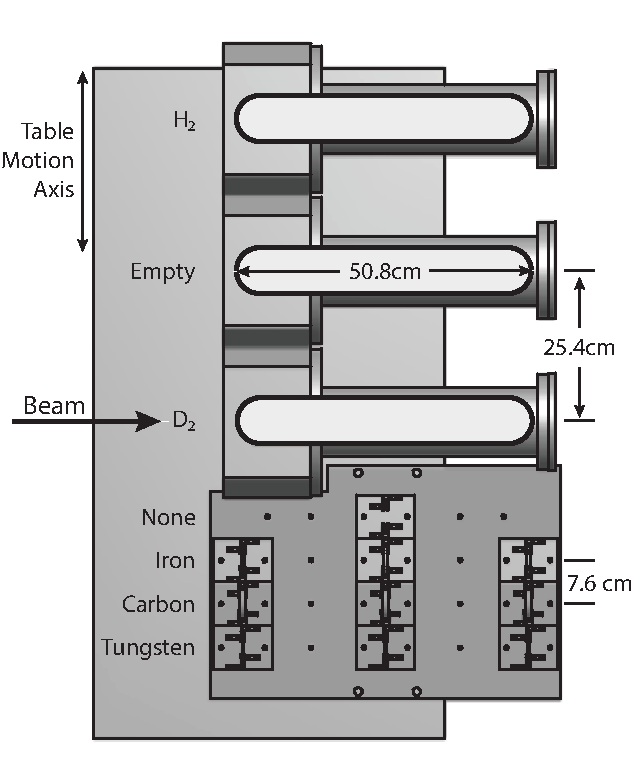
\includegraphics[width=\linewidth]{spectrometer/target-tableLayout.pdf}
	\caption{Schematic top view of the SeaQuest target table.}
	\label{fig:target_table}
\end{figure}
\begin{table}[h!]
	\centering
	\caption{Density and thickness of the target material and number of spills per target-rotation cycle for the SeaQuest targets.}
	\label{table:target}
	\begin{adjustbox}{max width=\linewidth}
		\begin{tabular}{ccccc}
			\hline \hline
			Material    & \makecell{Density\\(\unit{\g\per\cm\cubed})} & \makecell{Length\\(\unit{\cm})} & \makecell{No.\,of Interaction\\Lengths}   & Spills/cycle \\ \hline
			\ce{H_2}    & \num{0.071}       & \num{50.8} & \num{0.069}  & 10 \\
			Empty Flask & -                 & -          & \num{0.0016} & 2  \\
			\ce{D_2}    & \num{0.1634}      & \num{50.8} & \num{0.115}  & 5  \\
			\hline \hline
		\end{tabular}
	\end{adjustbox}
\end{table}
\subsection{Spectrometer}
\begin{figure*}
	\centering
	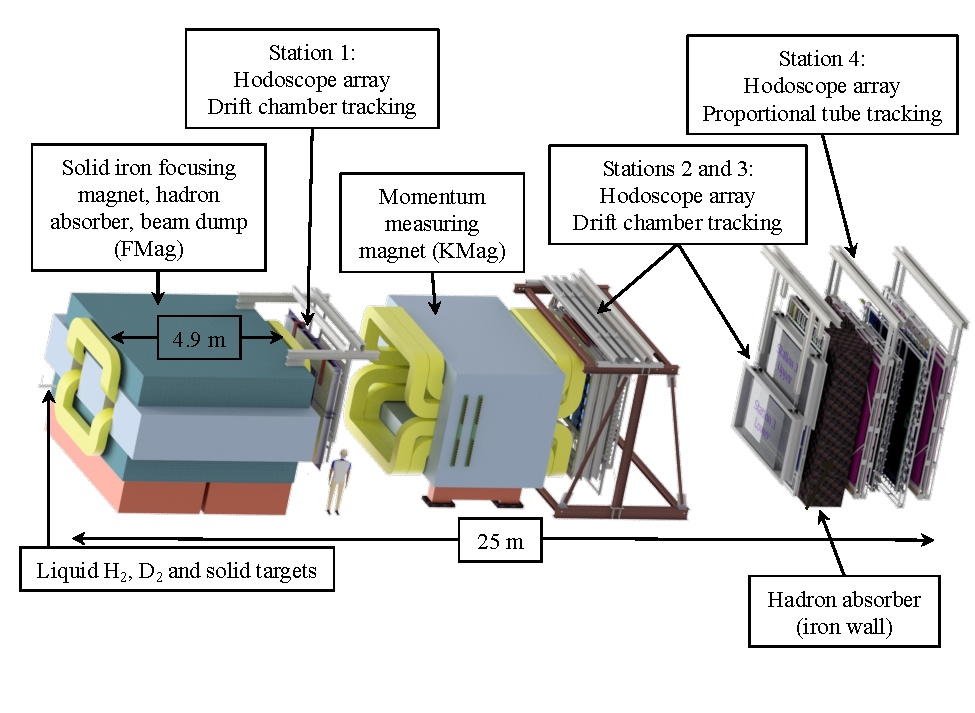
\includegraphics[width=0.8\linewidth]{spectrometer/twoColumnSeaQuestSpectrometerNIM.pdf}
	\caption{Schematic of the SeaQuest spectrometer.}
	\label{fig:spectrometer}
\end{figure*}
The schematic layout of the SeaQuest spectrometer, discussed in detail in Ref.~\cite{aidala2019},
is displayed in \cref{fig:spectrometer}.
The SeaQuest spectrometer consists of two magnets and four tracking stations.
A solid iron magnet,
FMag, is placed \SI{104}{\cm} downstream the target. It is then followed by
the first tracking station. The SeaQuest detector system is separated into four tracking stations.
Stations~1, 2 and 3 each consists of plastic scintillator hodoscopes and drift chambers.
The hodoscopes in each stations provides a fast signal for triggering whereas
the drift chambers provide good spatial resolution for precise track reconstruction.
An open air dipole magnet (KMag) is placed between station~1 and station~2.
Downstream of station~3, there is an \SI{1}{\meter} iron wall acting as an
absorber. Station~4 is located behind the  absorber and acts as a
muon identifier. Station~4 consists of a hodoscope array and 4 layers of
proportional tube planes.

\subsection{Trigger System}
The SeaQuest trigger uses discriminated signals from the hodoscope counters.
During SeaQuest data taking, there are five trigger inputs, but for this present analysis,
only two triggers are used, as listed in \cref{tab:triggers}.
Trigger~1 is the main physics trigger, and requires a coincidence of two opposite sign muons,
one in the top and one in the bottom halves of the spectrometer.
Trigger~4 only requires one muon track, and it is mainly used for studying the accidental background.
\begin{table}[tb]
	\centering
	\caption{Triggers used in the present analysis. The T or B denotes the top or bottom section traversed by the track. \label{tab:triggers}}
	\begin{tabular}{c@{\hspace{6\tabcolsep}}c@{\hspace{6\tabcolsep}}c@{\hspace{6\tabcolsep}}l}
		\hline
		\hline
		Trigger & Side  & Charge  & Description        \\
		\hline
		1       & TB/BT & $+-/-+$ & Unlike-sign dimuon \\
		4       & T/B   & $+/-$   & Single muon        \\
		\hline
		\hline
	\end{tabular}
\end{table}

\section{Data Analysis}
\label{sec:analysis}
\todo{progress between nature paper and now?}
The analysis procedure is largely similar to that described in Ref.~\cite{dove2023}.
\subsection{Track reconstruction}
The muon tracks are reconstructed using the hits in the drift chambers and proportional tubes in each stations. 
To reduce the number of potential hits, several catagories of spurious hits are first removed.
These include out-of-time hits, after-pulse hits, and cluster hits.
The out-of-time hits have a drift time outside of the allowable range;
The after-pulse hits are caused by occasional ringing in the readout electronics;
And the cluster hits are caused by $\delta$ rays or cosmic rays traveling parallel to the detector planes,
resulting in three or more hits in adjacent wires. 
The numbers of hits are further reduced by only preserving hits that correspond to a matching hodoscope hits.

After removing these hits, the remaining chambers hits are organized into straight-line segments (called tracklets)
for each of the first three stations.
The tracklets from different stations are then matched to find valid tracks consistent with muons 
originating from target area. 
The tracks are also projected to the proportional tubes in station~4, located after the iron absorber,
to identify corresponding hits and for muon identification.
The Kalman filter algorithm~\cite{kalman1960} are then used to further refine the muon tracks,
and determine the best estimate of the muon momentum.
The magnetic field of the two magnets and the energy loss in the solid iron FMag are also taken into account during this stage.
Finally, pairs of opposite charged muons tracks from the top and bottom sections of the spectrometer are
matched to determine the interaction vertex using Kalman filter.

\subsection{Monte Carlo simulation}
\label{subsec:MC}
\todo{Explain the event generation, geat4 options, embeding(?), realization(?).}
\todo{How well is our data discribed by GMC? Which distributions are we comparing?}

To compare the experimental results with theoretical expectations,
a GEANT4~\cite{agostinelli2003,allison2006,allison2016} based Monte Carlo simulations has been developed.
The Drell-Yan event generator is produce a uniform distribution in mass and $x_F$,
with weights proportional to the theoretical cross section, calculated using CT14 PDFs~\cite{hou2018}.
The dimuon transverse momentum distribution has been tunned to match the measured distribution.
Other PDFs, such as the statistical model~\cite{soffer2019}, were used to measure the systematic effects due to input PDFs.
The SeaQuest spectrometer is modeled and trajectories of the muons are calculated using GEANT4.
The energy loss and multiple scattering in the FMag are also included in the simulation,
and are the dominant factor in determining the momentum resolution of the muons. 

The efficiency and the resolution of the chambers are taken into account in the simulation
by dropping a small number of hits, and applying Gaussian smearing to the drift distance of the remaining hits.
Both the efficiency and the width of the smearing are taken from the data.

To simulate the noise and background hits during data taking,
each Monte Carlo events are embedded with hits recorded by the random trigger.
This allows us to determine the our reconstruction efficiency due to the varying chamber occupancies.
It also allows us to evaluate the accuracy of the reconstruction algorithm in measuring the dimuon kinematics.


\subsection{Mass-fit method}
\todo{Explain the method. If we are using NMSU mix, we will need to justify the normalization.}
The mass spectrum, as shown in \cref{fig:massfit} can be expressed as a linear combination of different components,
namely Drell-Yan, charmonium decays, accidental background and background from instruments.
These different contributions would have distinct mass spectra, for example, the $J/\psi$
and $\psi^\prime$ decays would have sharp distributions centered around their masses.
Therefore, the data can be fitted to various templates to obtain
the relative contribution from each sources. 
As input parameters to the fit, the mass distributions for $J/\psi$, $\psi\left(2S\right)$ 
and the Drell-Yan are obtained from studying the Monte Carlo simulation, as discussed in \cref{subsec:MC}.
The spectrum of accidental coincidence events was made by pairing at random $\mu^+$ and $\mu^-$ collected with the ``single-muon'' trigger (trigger 4 of \cref{tab:triggers})
under the condition that the beam intensities of $\mu^+$ and $\mu^-$ events were comparable.
The magnitudes of these components,
with the exception of the empty-flask data for which the normalization is known,
were varied in the fit to the mass spectrum.
The statistical uncertainties of the Monte Carlo and empty-flask date are taken into account using the algorithm described in Ref.~\cite{barlow1993}.
\Cref{fig:massfit} shows the fit to the $p+p$ and $p+d$ dimuon spectra respectively.
\begin{figure}[htbp!]
	\centering
	\begin{subfigure}{\linewidth}
		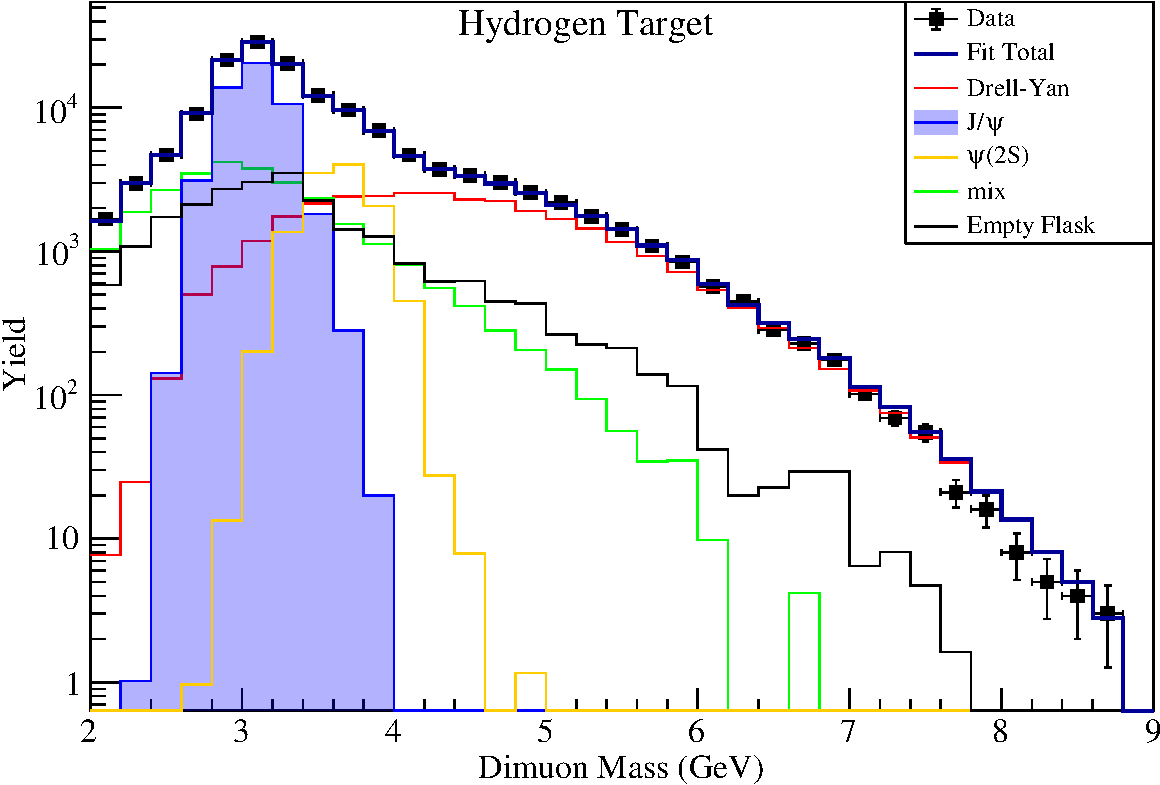
\includegraphics[width=\linewidth]{massfit_run56_LH2.pdf}
	\end{subfigure}
	\begin{subfigure}{\linewidth}
		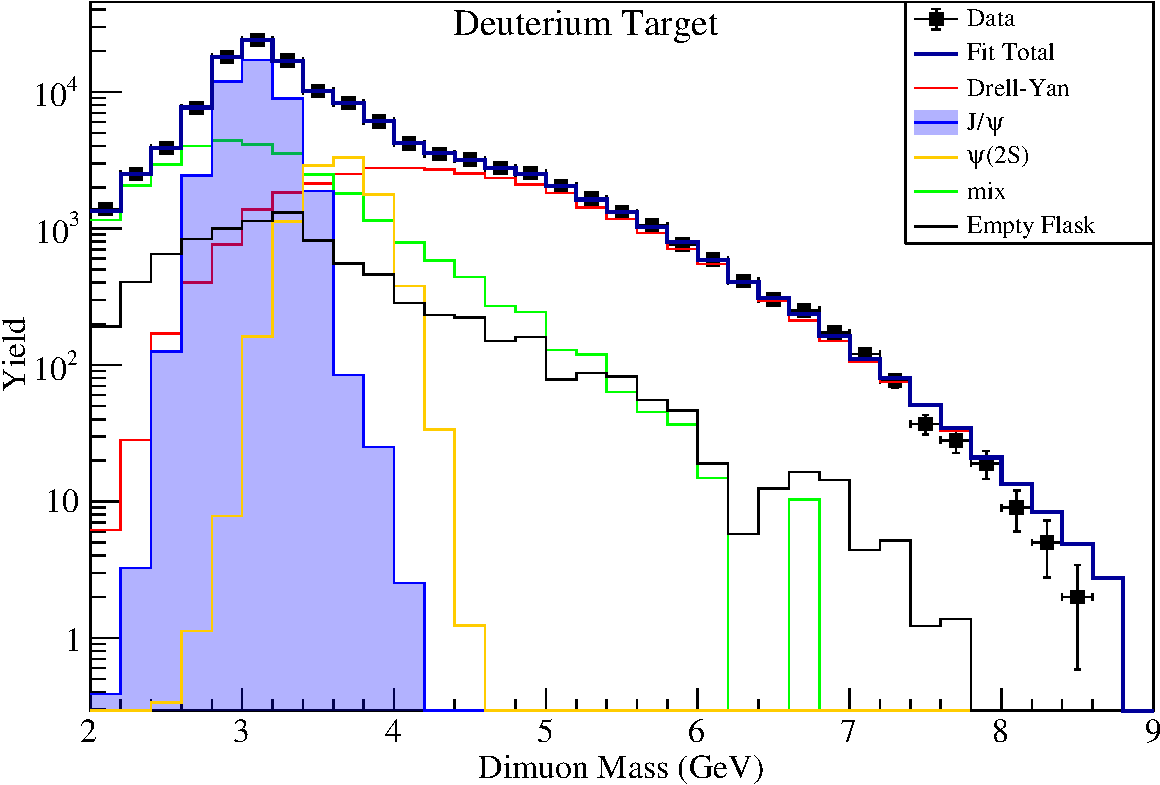
\includegraphics[width=\linewidth]{massfit_run56_LD2.pdf}
	\end{subfigure}
	\caption{Dimuon mass distribution for events collected
		on liquid hydrogen (top) and deuterium (bottom) targets for the second data set.
		The data points (solid squares) are compared with a fit (solid blue line) consisting of
		various components (see text).}
	\label{fig:massfit}
\end{figure}
\missingfigure[figwidth=\linewidth]{Drell-Yan yeild vs $x_T$ after background subtraction compared with MC}
\todo{corrections(?): rate dependence, target contamination, live PoT}
After the mass fit is performed, and the normalization for accidental background has been determined,
a mass cut ($M>\SI{4.5}{\GeV}$) is applied to remove the $J/\psi$ and $\psi\left(2S\right)$ events.
The remaining events are projected into various kinematic variables, such as $x_1$, $x_2$, $x_F$, and $P_T$.
Several corrections are applied to extract the final Drell-Yan yields.
These include the effective luminosity, obtained from the total number of protons on targets passing the BIM cut.
A target contamination correction is also applied to the \ce{D_2} data due to \ce{H} contamination in the target cell.
It should noted that during this analysis,
a revised correction is used as compared with the earlier work~\cite{dove2021,dove2023},
resulting in a roughly \SI{2}{\percent} shift in the ratios.
The reconstruction inefficiency and DAQ deadtime, which have a small but non-negligible target dependence,
are also taken into account.


\section{Measurement of The \texorpdfstring{$\sigma_{pd}/2\sigma_{pp}$}{pd/2pp} Drell-Yan Cross Section Ratio}
\label{sec:csr}
\todo{which variables do we want to show? (x2, x1, mass, pT, xF, etc)}
\Cref{fig:xT_csr} shows the measured $\sigma_{pd}/2\sigma_{pp}$ cross section ratio from the combined analysis
compared with results from E866~\cite{towell2001} and NLO calculations using DYNNLO~\cite{catani2007,catani2009},
with nucleon PDFs CT18~\cite{hou2021}. The measured ratio is also tabulated in \cref{tab:dbarubar}.
\Cref{subfig:xT_csr_data} shows the comparisons of the two datasets from SeaQuest.
The results from both data sets mostly consistent with each other, except for the low $x_2$ bin where our acceptance is smaller. 
And the results from the combined analysis is compared with results from E866~\cite{towell2001} in \cref{subfig:xT_csr_exp}.
As the E866 data is used in the CT18 global analysis, the small $x$ behavior in the PDF is well constrained. 
The consistence between the SeaQuest results and the CT18 calculations at small $x_2$ demonstrate the agreement between
the two experiments at this region.
The small difference between E866 and SeaQuest results between $0.1<x_2<0.2$ mostly originates from the different beam energies
and thus different $x_1$ coverage, as reflected in the calculated cross section ratios. 
At $x_2$ increases, the ratio measured by SeaQuest remains above one, and unlike E866, no drop off in the ratio is observed.
\begin{figure}[htbp!]
	\captionsetup[subfigure]{labelformat=empty}
	\begin{subfigure}{\linewidth}
		\centering
		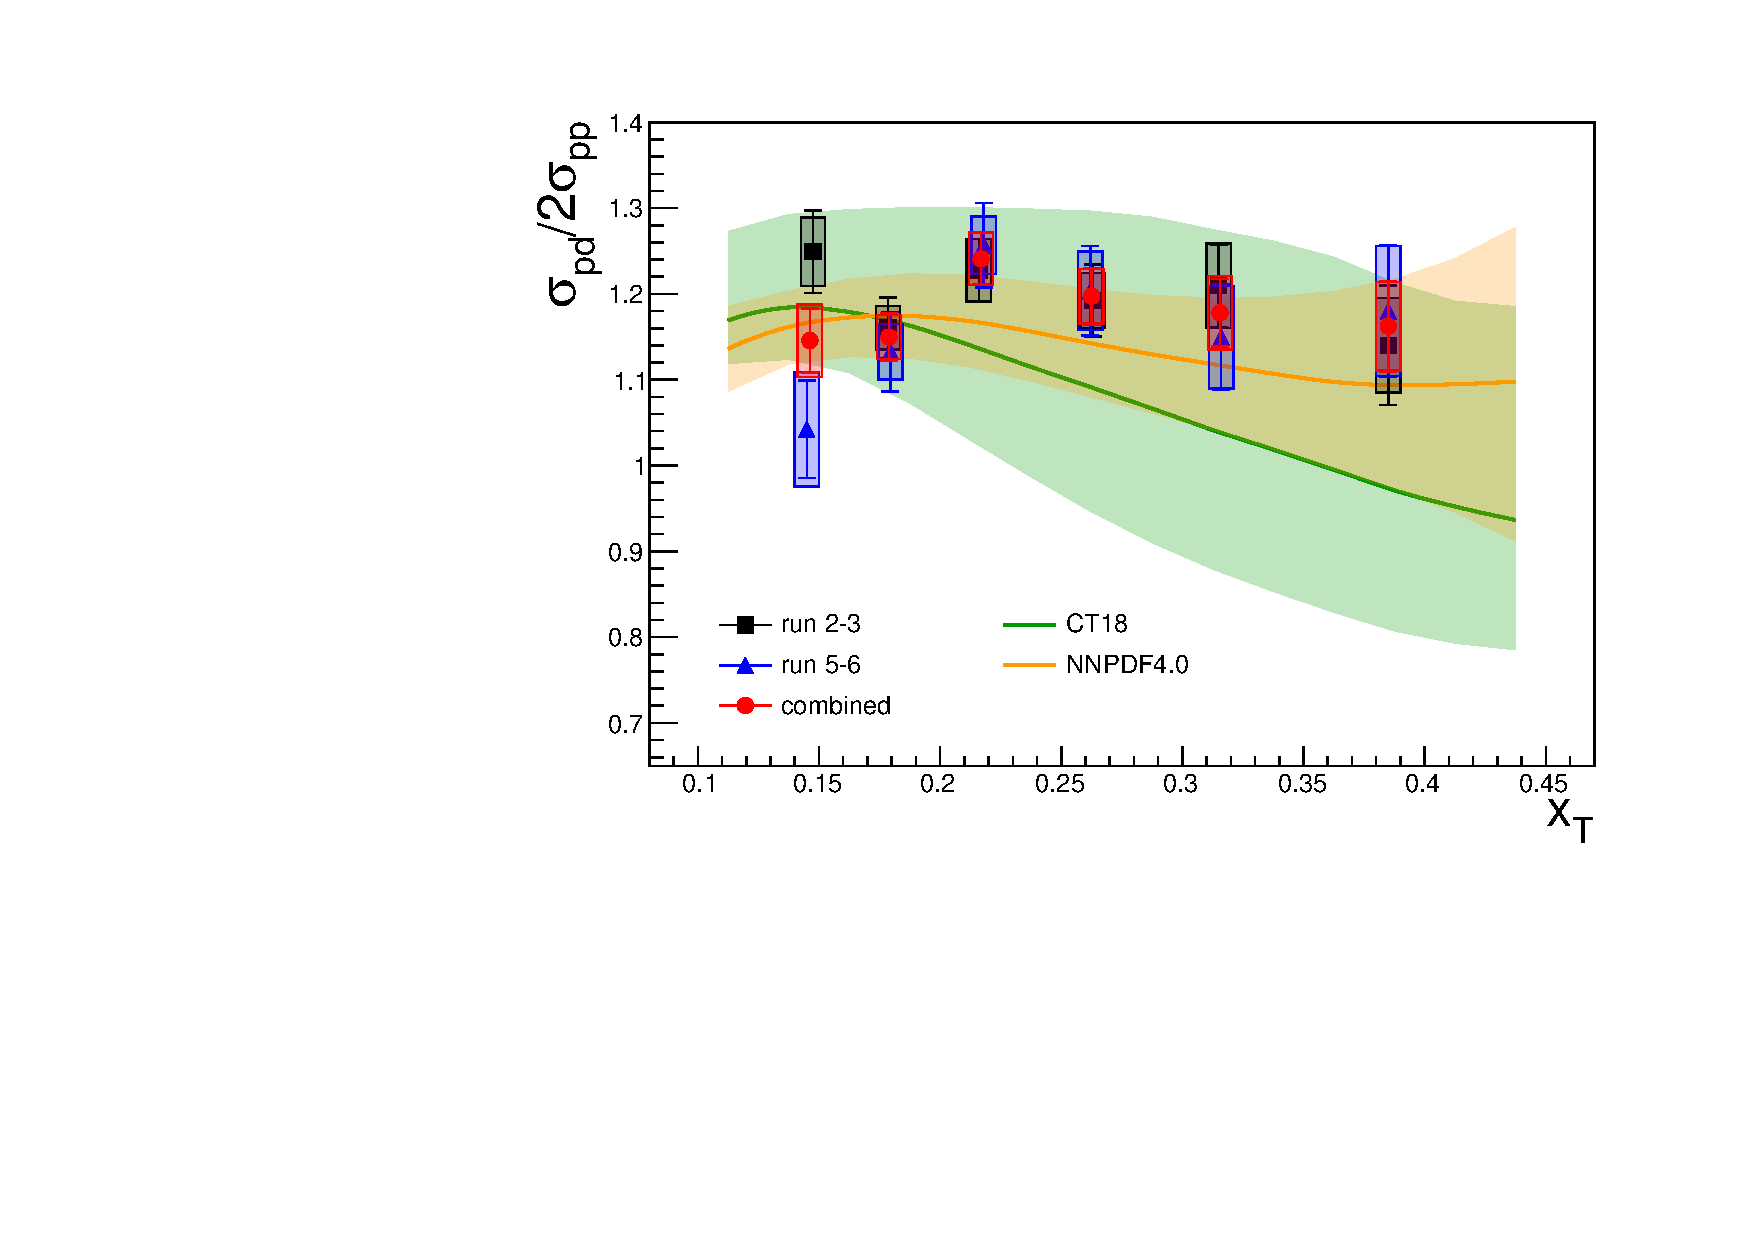
\includegraphics[width=\linewidth]{data_full_xT_syst.pdf}	
		\phantomcaption
		\label{subfig:xT_csr_data}
	\end{subfigure}
	\begin{subfigure}{\linewidth}
		\centering
		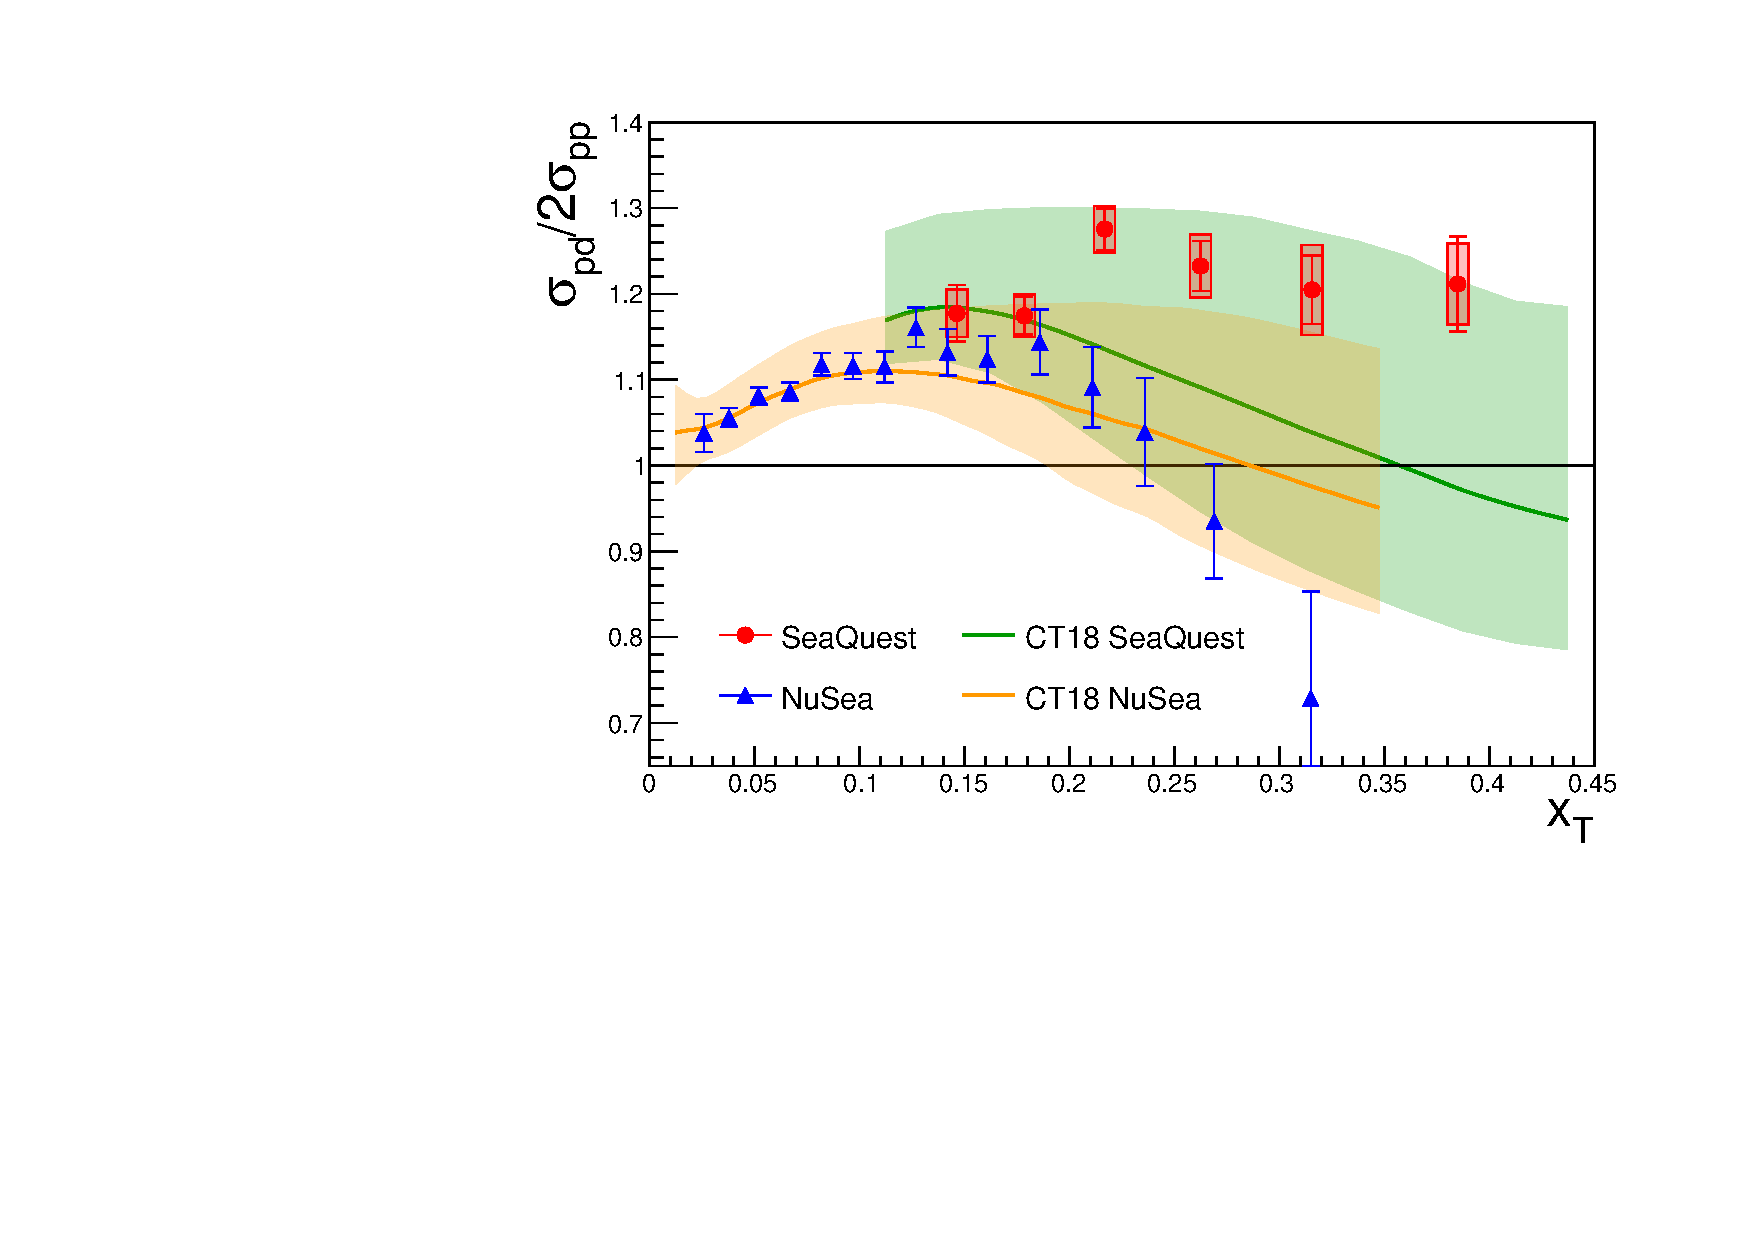
\includegraphics[width=\linewidth]{E906_E866_xT_CT18only.pdf}
		\phantomcaption
		\label{subfig:xT_csr_exp}
	\end{subfigure}
	\caption{Measured $\sigma_{pd}/2\sigma_{pp}$ Drell-Yan cross section ratio from the two SeaQuest datasets compared calculations using 
		CT18 ~\cite{hou2021} and NNPDF4.0~\cite{ball2022a} (top). As well as comparisons with
		with E866/NuSea~\cite{towell2001} and calculations using CT18~\cite{hou2021} at different kinematics (bottom).}
	\label{fig:xT_csr}
	\todo{which PDFs to use?}
\end{figure}
This strongly suggest the $\bar{d}/\bar{u}$ ratio to remain above unity at large $x$.

\todo{break down of systematics}
The sources of systematic uncertainties are tabulated in \cref{tab:sys_csr}.
The main uncertainties originate from the modeling of the accidental background ($\delta_{mix}$). 
Different methods for generating the accidental background distributions have been studied~\cite{pate2023},
and the differences are quoted as the systematic uncertainty.
Other sources of systematic uncertainties include the the efficiency corrections ($\delta_{Eff.\,stat.}$ and $\delta_{Eff.\,param.}$),
empty flask normalization ($\delta_{Empty}$), and the relative beam luminosity ($\delta_{Beam\,norm.}$).
\begin{table*}
	\centering
	\caption{Breakdown of systematic uncertainty for $\sigma_{pd}/2\sigma_{pp}$ ratio in each $x_2$ bins.}
	\label{tab:sys_csr}
	\begin{adjustbox}{max width=\linewidth}
		\begin{tabular}{c|cccccc}
\hline\hline
$x_2$                      & $0.13-0.16$         & $0.16-0.195$        & $0.195-0.24$        & $0.24-0.29$         & $0.29-0.35$         & $0.35-0.45$         \\ \hline
$\sigma_{pd}/2\sigma_{pp}$ & $1.177\pm0.033$     & $1.174\pm0.022$     & $1.275\pm0.024$     & $1.232\pm0.029$     & $1.205\pm0.040$     & $1.212\pm0.055$     \\ \hline
$\delta_{Eff.\,stat.}$     & \SI{0.57}{\percent} & \SI{0.37}{\percent} & \SI{0.36}{\percent} & \SI{0.41}{\percent} & \SI{0.51}{\percent} & \SI{0.69}{\percent} \\
$\delta_{Eff.\,param.}$    & \SI{0.41}{\percent} & \SI{0.28}{\percent} & \SI{0.46}{\percent} & \SI{0.27}{\percent} & \SI{0.26}{\percent} & \SI{0.27}{\percent} \\
$\delta_{Mix}$             & \SI{1.00}{\percent} & \SI{0.48}{\percent} & \SI{0.41}{\percent} & \SI{2.17}{\percent} & \SI{3.82}{\percent} & \SI{3.23}{\percent} \\
$\delta_{Empty}$           & \SI{0.14}{\percent} & \SI{0.10}{\percent} & \SI{0.16}{\percent} & \SI{0.15}{\percent} & \SI{0.13}{\percent} & \SI{0.15}{\percent} \\
$\delta_{Beam\,norm.}$     & \SI{2}{\percent}    & \SI{2}{\percent}    & \SI{2}{\percent}    & \SI{2}{\percent}    & \SI{2}{\percent}    & \SI{2}{\percent}    \\ \hline
$\delta_{syst.}$           & $\pm 0.028$         & $\pm 0.025$         & $\pm 0.027$         & $\pm 0.037$         & $\pm 0.052$         & $\pm 0.047$         \\ \hline\hline
\end{tabular}

	\end{adjustbox}
\end{table*}
\todo{consistence of the data(source of systematics)}

\section{Extraction of \texorpdfstring{$\bar{d}\left(x\right)/\bar{u}\left(x\right)$}{dbar(x)/ubar(x)}
  and \texorpdfstring{$\bar{d}\left(x\right)-\bar{u}\left(x\right)$}{dbar(x)-ubar(x)}}
\label{sec:extraction}
\todo{Explain the extraction. There are also addition systematics here.}
\todo{Where to put acceptance? We did show the acceptance in nature paper.}
In order to compare the results from SeaQuest with predictions from various models,
an estimate for the $\bar{d}/\bar{u}$ ratio is extracted from the cross section ratio by
an iterative method, as described in Ref.~\cite{dove2021}.
We first make an estimate for the $\bar{d}/\bar{u}$ ratio over the measured $x_2$
and calculate the cross section ratio $R$ using a chosen PDF set.
This PDF set provides all other parton distributions except for the $\bar{d}/\bar{u}$ ratio,
which is allowed to vary. The $\bar{d}/\bar{u}$ ratio is initialized as
\begin{equation}
	\left[\frac{\bar{d}}{\bar{u}}\right]\left(x_2\right) = 2R\left(x_2\right)-1.
\end{equation}
The $\bar{d}/\bar{u}$ ratio outside the measured $x_T$ range was assumed to be $1.0$,
and changed to $0.5$ and $2.0$ to estimate the systematic uncertainty arises from this assumption.
The cross section ratio $R$ is then calculated up to next-to-leading order, as
\begin{equation}
	R_{\mathrm{pred}}\left(x_T\right)  = \frac{\sum_{x_1} A\left(x_1, x_2\right)\sigma^{pd}_{NLO}\left(x_1, x_2\right)}{2\sum_{x_1} A\left(x_1, x_2\right)\sigma^{pp}_{NLO}\left(x_1, x_2\right)},
\end{equation}
where $A\left(x_1,x_2\right)$ is the acceptance for a $\left(x_1, x_2\right)$ bin.
The $\bar{d}/\bar{u}$ ratio is then adjusted according to the difference between
the measured and predicted ratios, until the difference is less than $10^{-3}$.

The extracted $\bar{d}/\bar{u}$ from the measured SeaQuest cross section ratio,
using the CT18 PDFs as the basis, are shown in \cref{fig:e906_e866_dbarubar}
and tabulated in \cref{tab:dbarubar}.
While the SeaQuest results are consistent with previous E866 results~\cite{towell2001} at low $x$,
the extracted $\bar{d}/\bar{u}$ ratios from the SeaQuest measurement continue to rise as $x$ increases,
and is in tension with the E866 result.
The SeaQuest results are also in much better agreement with predictions from meson cloud model~\cite{alberg2022}
and statistical model~\cite{soffer2019}.
The extracted $\bar{d}/\bar{u}$ ratios are also compared with results from CT18~\cite{hou2021} and NNPDF4.0~\cite{ball2022a}
global analyses in \cref{fig:e906_e866_dbarubar}.
The inclusion of the SeaQuest result from Run 2-3 in the NNPDF4.0 analysis strongly constrains the $\bar{d}/\bar{u}$ ratios
to remain above unity at large $x$.
With the reduced statistical uncertainties from the combined analysis presented in this thesis,
the uncertainty on the $\bar{d}/\bar{u}$ in these global analyses can be further reduced.

\begin{table*}[htbp!]
	\centering
	\caption{The measured $\sigma_{pd}/2\sigma_{pp}$ cross section ratio as well
		as the extracted $\bar{d}/\bar{u}$ and $\bar{d}-\bar{u}$ for each $x_{2}$ bin.
		The first uncertainty is statistical and the second systematic.}
	\label{tab:dbarubar}
	\begin{adjustbox}{max width=\textwidth}
		% !TeX root = ../main.tex
{
\renewcommand{\arraystretch}{1.5}
\begin{tabular}{cccccccc}
	\hline\hline
	$x_{2}$ range    & $\expval{x_{2}}$ & $\expval{x_{1}}$ & $\expval{p_{T}}(\unit{\GeV/c})$ & $\expval{M}(\unit{\GeV/c^2})$ & $\sigma_{pd}/2\sigma_{pp}$ & $\bar{d}/\bar{u}$                     & $\bar{d}-\bar{u}$                     \\ \hline
	$0.130$--$0.160$ & $0.146$          & $0.687$          & $0.760$                         & $4.71$                        & $1.177\pm0.033\pm0.028$    & $1.383^{+0.058+0.060}_{-0.053-0.060}$ & $0.176^{+0.021+0.024}_{-0.022-0.023}$ \\
	$0.161$--$0.201$ & $0.181$          & $0.610$          & $0.759$                         & $4.87$                        & $1.174\pm0.022\pm0.025$    & $1.431^{+0.041+0.061}_{-0.051-0.061}$ & $0.111^{+0.011+0.011}_{-0.011-0.011}$ \\
	$0.202$--$0.242$ & $0.222$          & $0.553$          & $0.760$                         & $5.11$                        & $1.275\pm0.024\pm0.027$    & $1.672^{+0.052+0.082}_{-0.052-0.082}$ & $0.092^{+0.012+0.012}_{-0.012-0.012}$ \\
	$0.243$--$0.293$ & $0.263$          & $0.516$          & $0.761$                         & $5.44$                        & $1.232\pm0.029\pm0.037$    & $1.653^{+0.073+0.123}_{-0.073-0.113}$ & $0.043^{+0.003+0.013}_{-0.003-0.013}$ \\
	$0.294$--$0.354$ & $0.324$          & $0.492$          & $0.762$                         & $5.83$                        & $1.205\pm0.040\pm0.052$    & $1.694^{+0.124+0.174}_{-0.114-0.174}$ & $0.024^{+0.004+0.004}_{-0.004-0.004}$ \\
	$0.355$--$0.455$ & $0.395$          & $0.474$          & $0.762$                         & $6.34$                        & $1.212\pm0.055\pm0.047$    & $1.925^{+0.205+0.205}_{-0.195-0.205}$ & $0.015^{+0.005+0.005}_{-0.005-0.005}$ \\ \hline\hline
\end{tabular}
}

	\end{adjustbox}
\end{table*}
\begin{table*}[htbp!]
	\centering
	\caption{Values of $\int_{0.45}^{0.13} \left[\bar{d}\left(x\right) - \bar{u}\left(x\right)\right] \dd{x}$
		and $\int_{0.45}^{0.13} x\left[\bar{d}\left(x\right) - \bar{u}\left(x\right)\right] \dd{x}$ at $Q^2=\SI{25.5}{\GeV\squared}$ extracted from
		SeaQuest compared with CT18, NNPDF4.0 PDFs as well as meson cloud and statistical models.}
	\label{tab:dbarMubar}
	\begin{adjustbox}{max width=\textwidth}
		% !TeX root = ../main.tex
\renewcommand{\arraystretch}{1.5}
\begin{tabular}{ccccccc}
\hline \hline
 &          & \multicolumn{2}{c}{PDFs} & & \multicolumn{2}{c}{Models} \\ \cline{3-4} \cline{6-7}
 & SeaQuest &CJ22     & NNPDF4.0     & & Stat.     & Meson cloud    \\ \hline
$\int^{0.45}_{0.13} \left[\bar{d}\left(x\right) - \bar{u}\left(x\right) \right]\dd{x}$ &
  $0.0179_{-0.0018}^{+0.0017} {}_{-0.0023}^{+0.0022}$ &
  $0.0167^{+0.0009}_{-0.0028}$ &
  $0.0208^{+0.0036}_{-0.0036}$ & &
  $0.0186$ &
  $0.0180$ \\
$\int^{0.45}_{0.13} x\left[\bar{d}\left(x\right) - \bar{u}\left(x\right) \right]\dd{x}$ &
  $0.00368_{-0.00036}^{+0.00034} {}_{-0.00049}^{+0.00045}$ &
  $0.00319^{+0.00019}_{-0.00063}$ &
  $0.00414^{+0.00078}_{-0.00078}$ & &
  $0.00386$ &
  $0.00361$ \\ \hline \hline
\end{tabular}

	\end{adjustbox}
\end{table*}

The isovector PDF $\bar{d}-\bar{u}$ over the region $0.13<x<0.45$
can also be calculated from the extracted $\bar{d}/\bar{u}$ ratio by taking the $\bar{d}+\bar{u}$
distribution from CT18.
As a flavor non-singlet quantity, the integral, $\int^1_0 \left[\bar{d}\left(x\right) - \bar{u}\left(x\right)\right] \dd{x}$,
is expected to be independent of $Q^2$, even though the $x$ dependence might differ at different $Q^2$.
As the perturbative processes should not produce a significant $\bar{d},\,\bar{u}$ difference,
the $\bar{d}-\bar{u}$ values can provide a direct measure on the non-perturbative contributions.
The values of $\bar{d}-\bar{u}$ derived from the SeaQuest data are shown in \cref{fig:e906_e866_dbarMubar} and tabulated in \cref{tab:dbarubar},
and are also compared with results from E866~\cite{towell2001} and HERMES~\cite{ackerstaff1998},
and with predictions from meson cloud and statistical models.
Unlike $\bar{d}/\bar{u}$ ratio, the difference $\bar{d}-\bar{u}$ is insensitive to the flavor-symmetric contributions
to the sea-quark distributions in these models. Like the ratio, the deduced difference $\bar{d}-\bar{u}$ is also
in good agreement with both models.
It is also worth pointing out that the small $x$ behavior of the $\bar{d}-\bar{u}$ can be studied using
semi-inclusive DIS as indicated by the HERMES measurements~\cite{ackerstaff1998}.
With the advent of the Electron Ion Collider, the flavor asymmetry at small $x$ region, where abundant sea-quarks reside,
can be further constrained.
The flavor asymmetry $\bar{d}-\bar{u}$ can also be study using lattice techniques
within the framework of LaMET.
Though, it has been pointed out that calculations from lattice in the antiquark region are currently
susceptible to systematic uncertainties,
and in particular the inverse problem arising in the reconstruction of the $x$-dependence~\cite{constantinou2021}.
The current results using the LaMET framework do not agree among different groups nor with current global PDF analyses.
The measured flavor asymmetry can provide an important benchmark for the lattice calculations in the future.

The SeaQuest data can also be used to calculate two integral: $\int^{0.45}_{0.13} \left[\bar{d}\left(x\right) - \bar{u}\left(x\right) \right]\dd{x}$,
which describes the integrated sea-quark flavor asymmetry, and $\int^{0.45}_{0.13} x\left[\bar{d}\left(x\right) - \bar{u}\left(x\right) \right]\dd{x}$,
which represents the difference in the momentum fractions carried by $\bar{u}$ and $\bar{d}$ quarks.
These values are listed in \cref{tab:dbarMubar}, and are compared with different PDFs and models.
It should be noted that as SeaQuest is only probing the large $x$ region, the sea-quark PDFs are small in this region.
Hence, when compared with the measured $\int^{1}_{0} \left[\bar{d}\left(x\right) - \bar{u}\left(x\right) \right]\dd{x}=0.118\pm 0.012$
from E866 based on the measurements over $0.015<x<0.35$ and extrapolations~\cite{towell2001},
the result from SeaQuest is inherently smaller.

\begin{figure}[htpb!]
	\centering
	\begin{subfigure}{\linewidth}
		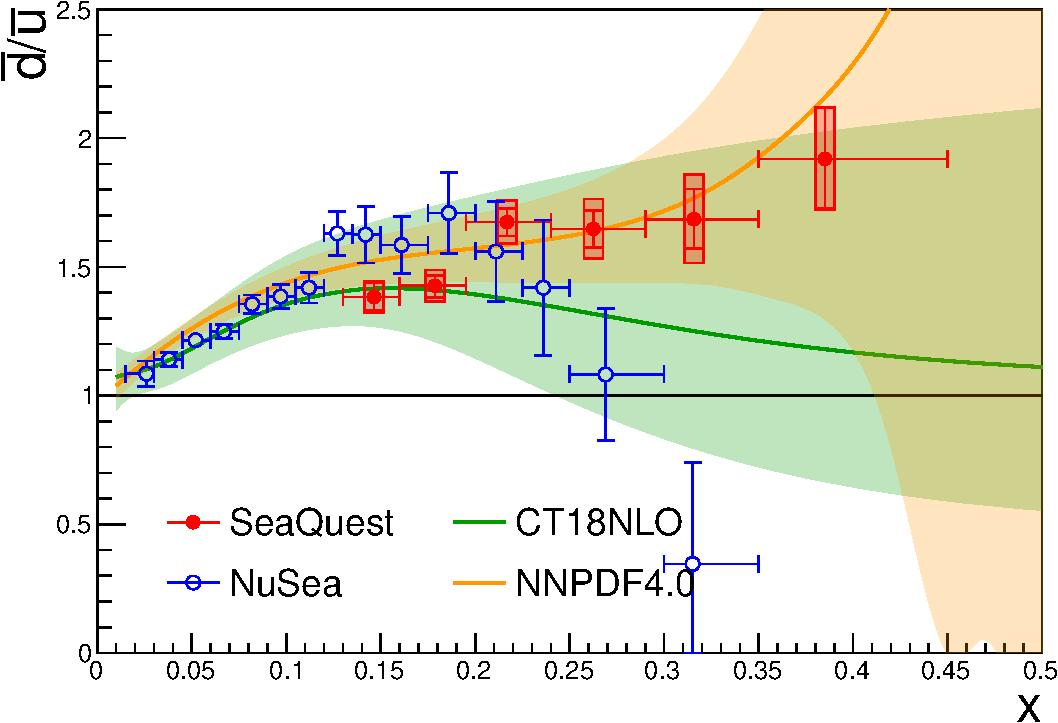
\includegraphics[width=\linewidth]{E906_E866_dbarubar_PDF.pdf}
	\end{subfigure}
	\begin{subfigure}{\linewidth}
		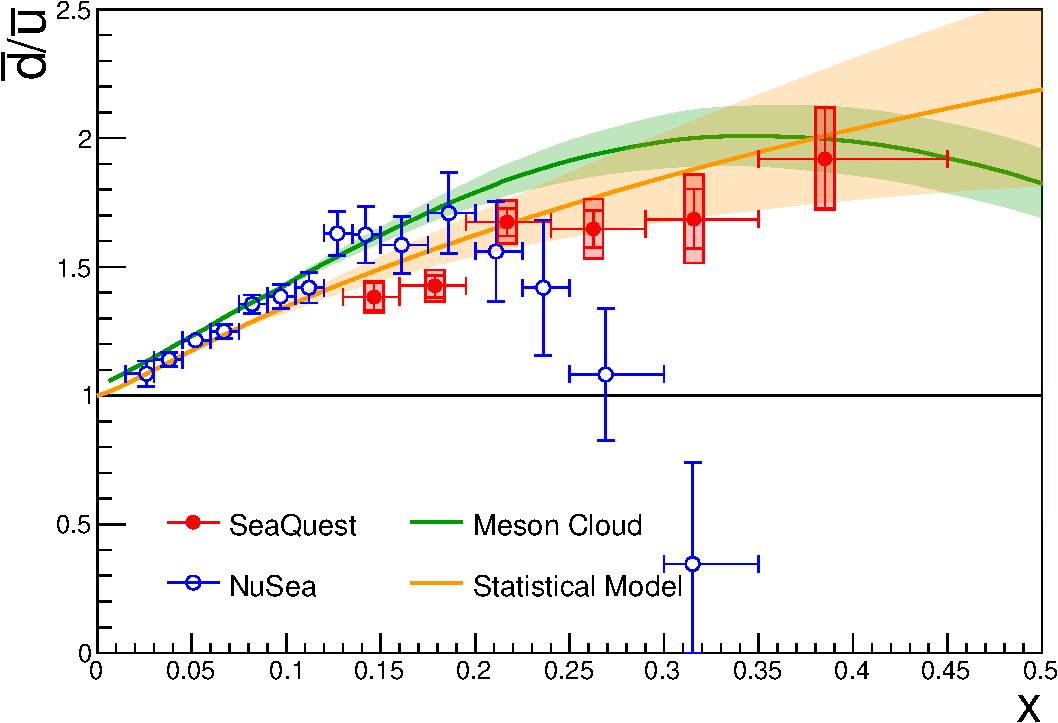
\includegraphics[width=\linewidth]{E906_E866_dbarubar.pdf}
	\end{subfigure}
	\caption{The extracted $\bar{d}/\bar{u}$ from the measured $\sigma_{pd}/2\sigma_{pp}$ Drell-Yan cross section ratio
		from SeaQuest (red solid circles), E866~\cite{towell2001} (open blue circles).
		The extracted ratios are compared with CT18~\cite{hou2021} and NNPDF4.0~\cite{ball2022a} global PDF analyses (top)
		and with predictions from meson cloud model~\cite{alberg2022} and statistical model~\cite{soffer2019} (bottom).}
	\label{fig:e906_e866_dbarubar}
\end{figure}

\begin{figure}[htpb!]
	\centering
	\begin{subfigure}{\linewidth}
		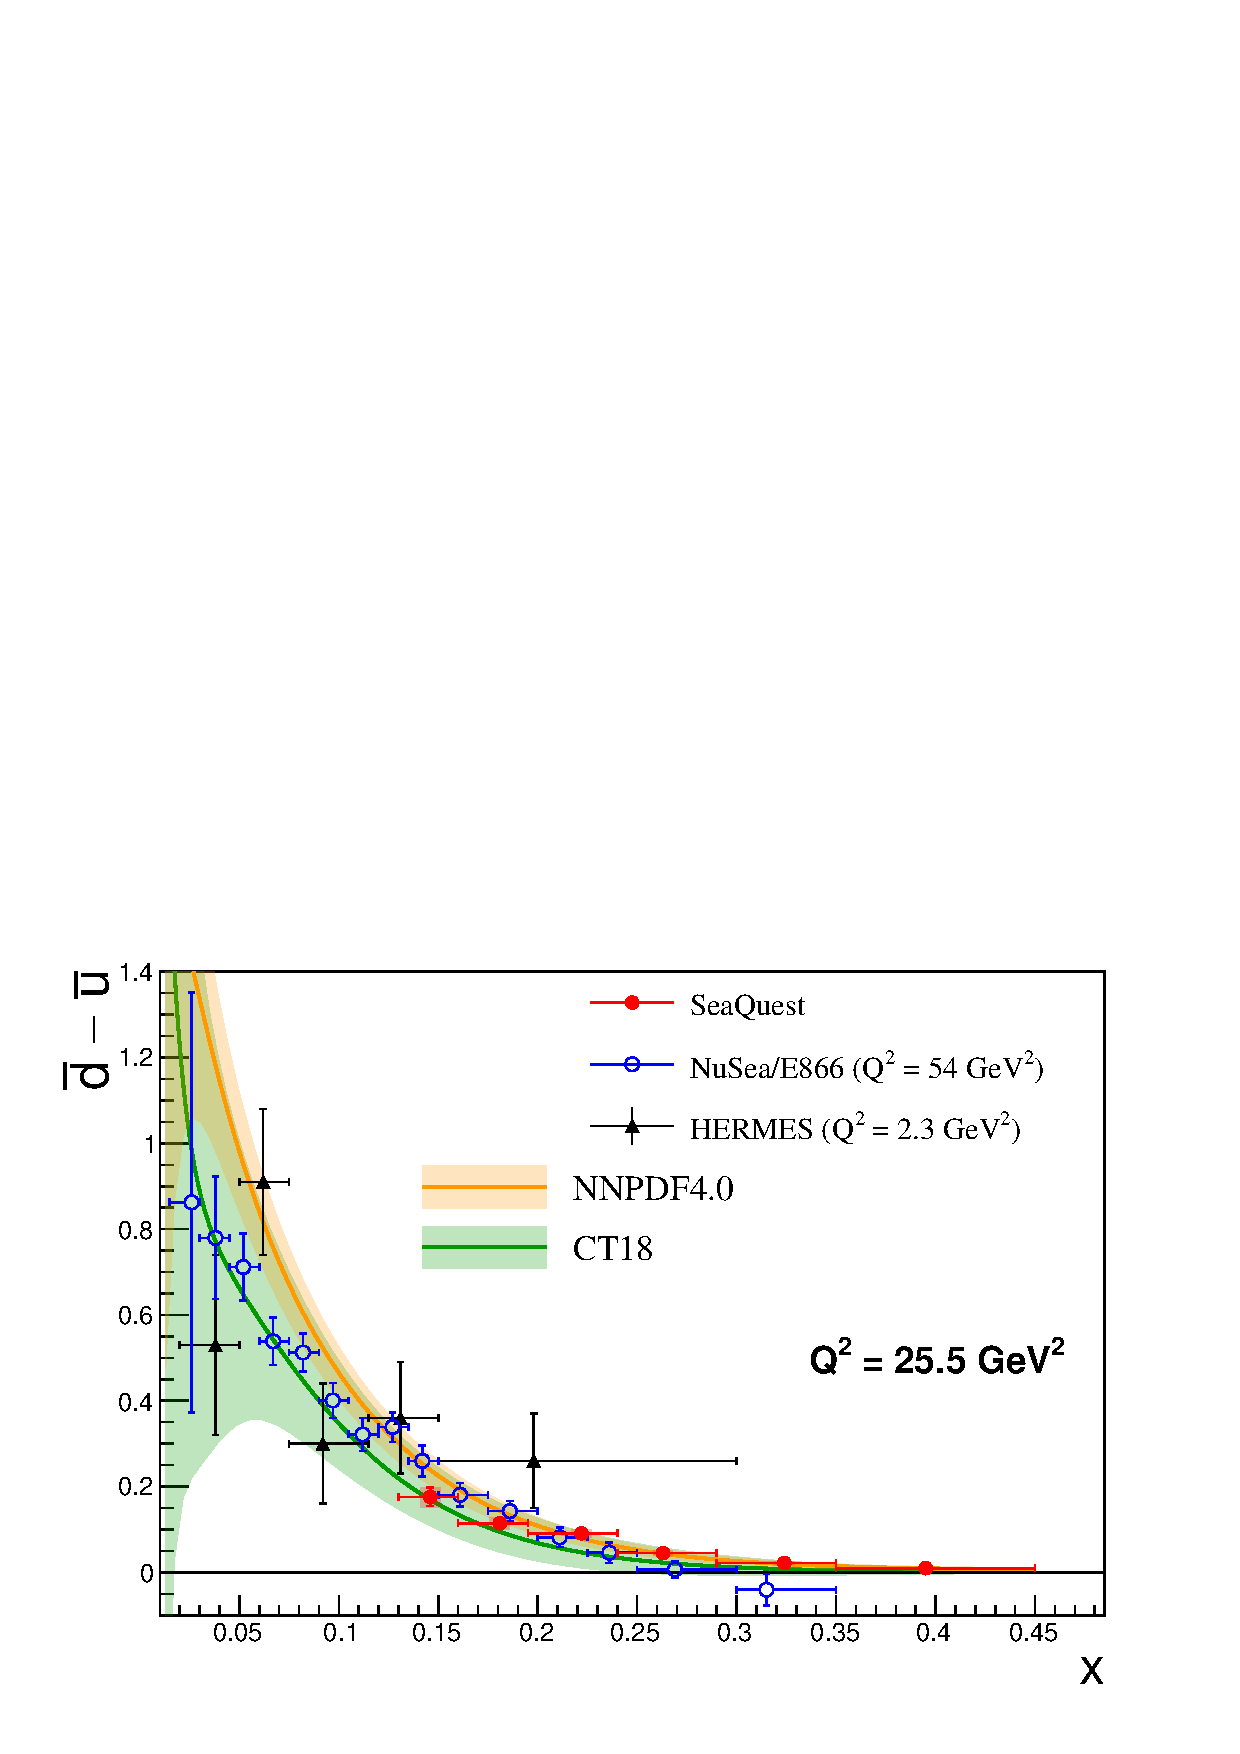
\includegraphics[width=\linewidth]{dbub_diff_with_PDF.pdf}
	\end{subfigure}
	\begin{subfigure}{\linewidth}
		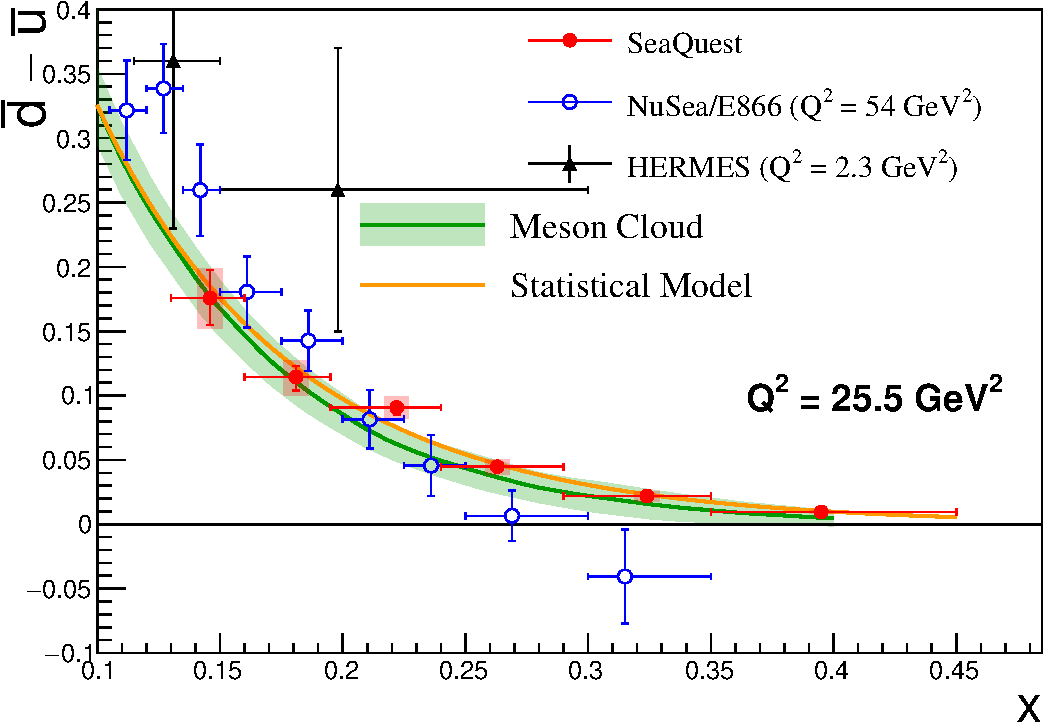
\includegraphics[width=\linewidth]{dbub_diff_with_model.pdf}
	\end{subfigure}
	\caption{The extracted $\bar{d}-\bar{u}$ from from SeaQuest (red solid circles), E866~\cite{towell2001} (open blue circles)
		and HERMES~\cite{ackerstaff1998} (black triangles).
		The results are compared with CT18~\cite{hou2021} and NNPDF4.0~\cite{ball2022a} global PDF analyses (top)
		and with predictions from meson cloud model~\cite{alberg2022} and statistical model~\cite{soffer2019} (bottom).
		The bottom panel is also zoomed in on $x>0.1$ in order to emphasis the SeaQuest results.}
	\label{fig:e906_e866_dbarMubar}
\end{figure}

\section{Measurement of \texorpdfstring{$p+p$}{p+p} and \texorpdfstring{$p+d$}{p+d} Drell-Yan cross section}
\label{sec:abs_cs}
\begin{figure*}
	\missingfigure{Drell-Yan cross section: pp and pd on two seperate pannel. All $x_F$}
	\caption{The $p+p$ (left) and $p+d$ (right) Drell-Yan double differential cross section $M^3d^2\sigma/dMdx_F$.
		The dotted curves are NLO calculations using NNPDF4.0~\cite{ball2022a} parton distribution functions.}
\end{figure*}
\todo{What are the discussion here? This part should be removed if this is a letter.}

\section{Impact on PDF analysis}
\todo{Not sure about this part}

\section{Conclusions}
\label{sec:Conclusions}
In summary, we have reported the improved results on the $\sigma_{pd}/2\sigma_{pp}$ Drell-Yen cross section ratio up to $x_2=4.5$,
based on the analysis of the entire SeaQuest dataset.
The measured ratio remains above unity, which suggests the $\bar{d}/\bar{u}$ ratio continues to increase at large $x$.
These results are in better agreement with various model predictions, including the meson cloud model and the statistical model.

\begin{acknowledgments}
	This work was performed by the SeaQuest Collaboration, whose work was supported in part by the
	\todo{Add funding information}
\end{acknowledgments}
\bibliography{reference}

\end{document}

